%Texlive-full Version 3.141592-1.40.3 (Web2C 7.5.6)
%Kile Version 2.0.83
%File associated : SoFa_Logo.ps , FF.ps

\documentclass[a4paper,10pt]{article}
\usepackage[utf8x]{inputenc}
\usepackage[T1]{fontenc} 

\usepackage{lmodern}
\usepackage[a4paper]{geometry}
%\usepackage[frenchb]{babel}
\usepackage{graphicx}
\usepackage{hyperref}

\usepackage{pstricks}
\usepackage{pst-node}
%\usepackage{wrapfig}
\usepackage{amsmath}
\usepackage{amsfonts}
\usepackage{amssymb}
\usepackage{textcomp}
%\usepackage{mathaccent}
\usepackage{listings}
\lstset{language=C++,basicstyle=\scriptsize \color{green},identifierstyle=\color{orange},keywordstyle=[1]\color{blue},columns=fullflexible,commentstyle=\textit}

\usepackage{color}



\begin{document}
%%%%%%%%%%%%%%%%%%   LOGO  %%%%%%%%%%%%%%%%%%%%%%%%%
\begin{center}
\rput(6,1.5){\href{http://www.sofa-framework.org/}{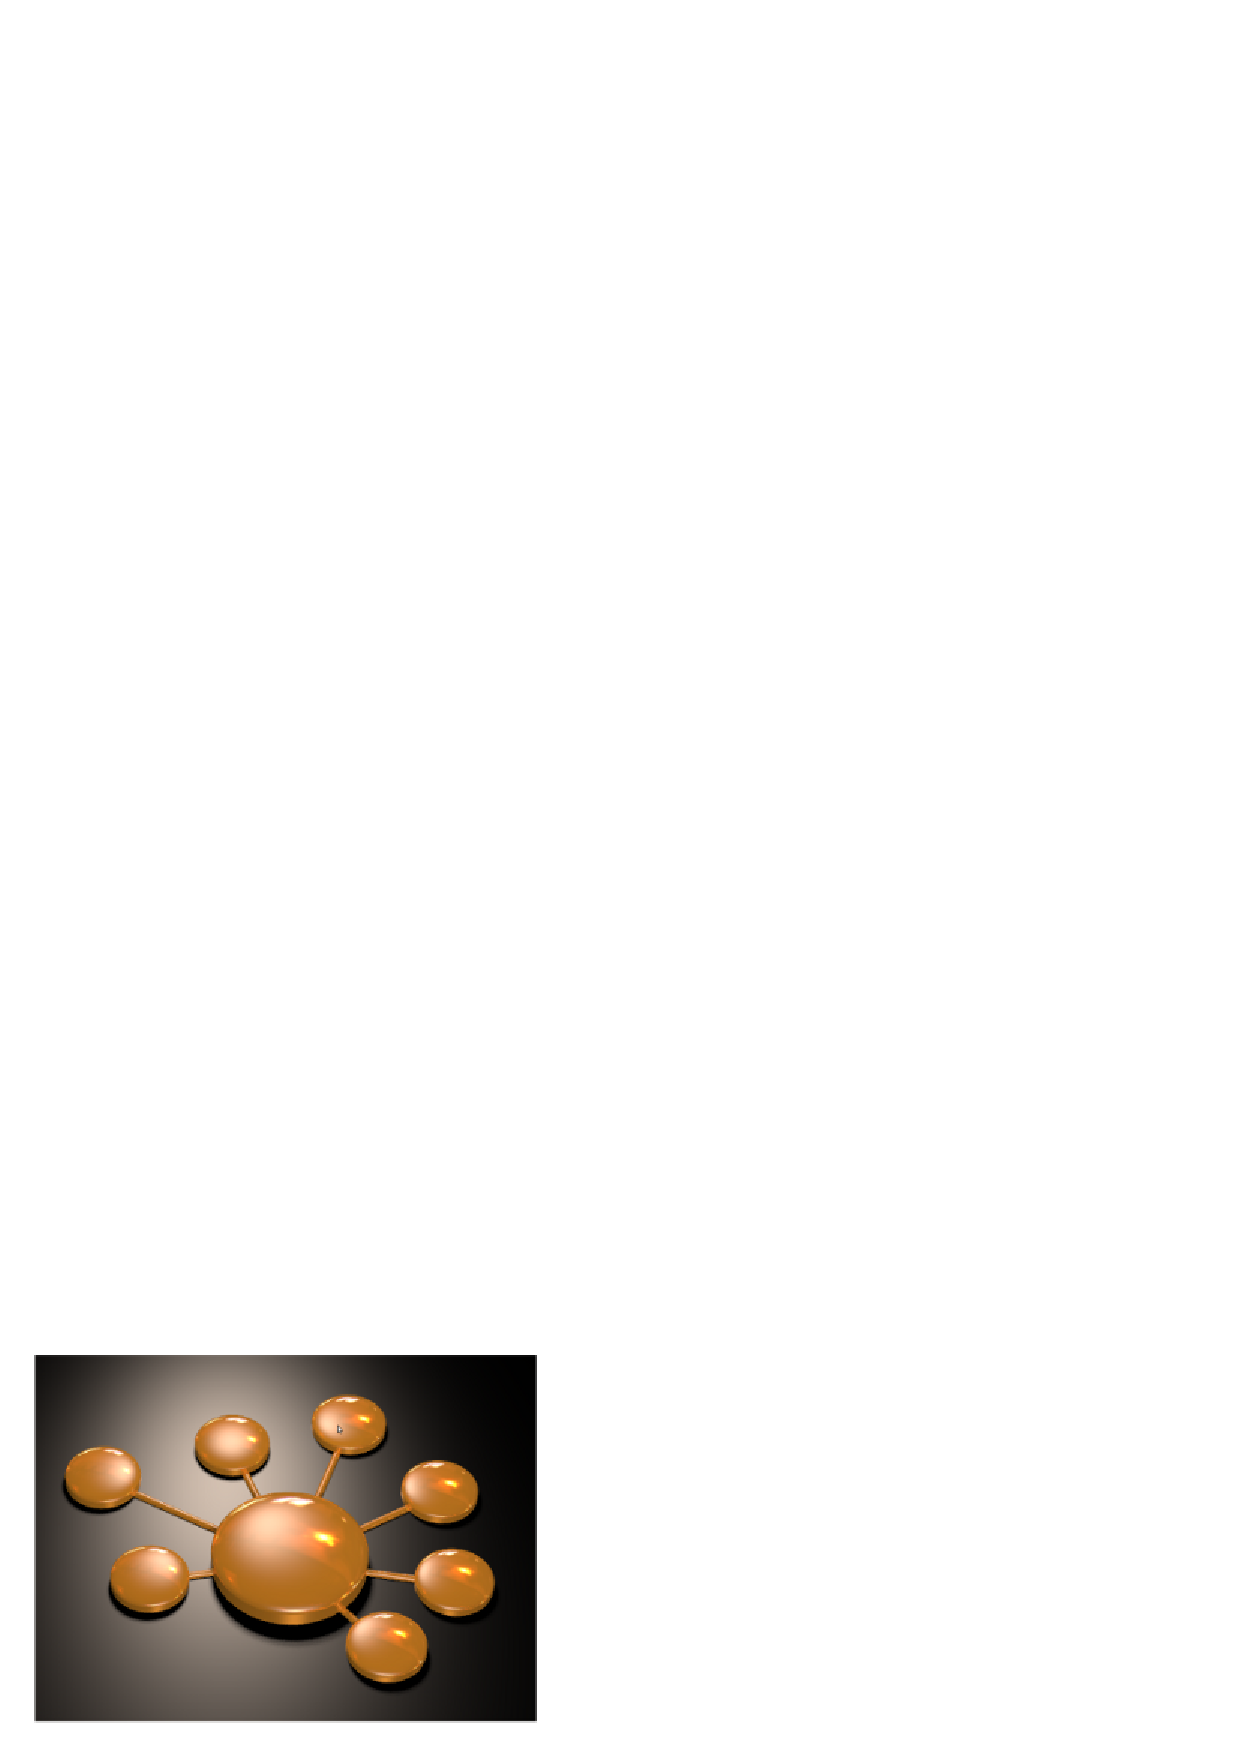
\includegraphics[scale=0.3]{SoFa_Logo}}}
\rput(-4,1.5){\href{http://www.sofa-framework.org/}{
		\begin{tabular}{l}
		\resizebox{4cm}{0.6cm}{SOFA} \\ 
		\resizebox{6cm}{0.3cm}{Simulation Open Framework Architecture}
		\end{tabular}
		}
	    }
\end{center}
%%%%%%%%%%%%%%%%%%   LOGO  %%%%%%%%%%%%%%%%%%%%%%%%%

%%%%%%%%%%%%%%%%%% DOCUMENT TITLE %%%%%%%%%%%%%%%%%%%%%%%%% To be deleted when include in the global document
%\chapter{Mapping} %\section{Rigid Mapping} 
\vspace{1.5cm}
\begin{center}\resizebox{7cm}{0.6cm}{Linear Solver}\end{center}
%%%%%%%%%%%%%%%%%% DOCUMENT TITLE %%%%%%%%%%%%%%%%%%%%%%%%%

%%%%%%%%%%%%%%%%%%%%%%%%%%%%%%%%%%%%%%%%%%%%%%%%%%%%%%%%%%%%%%%%%%%%%%%%%%%%%%%%%%%%%%%%%
%=======================================================================================%
%%%%%%%%%%%%%%%%%%%%%%%%%%%%%%%%%%%%%%%%%%%%%%%%%%%%%%%%%%%%%%%%%%%%%%%%%%%%%%%%%%%%%%%%%
%\section{Linear Solver}% for adding to the global document of SOFA

\section{Linear Solver}
\paragraph{Abstract : }
%%%%%%%%%%%%%%%%%%   LOGO  %%%%%%%%%%%%%%%%%%%%%%%%%
%%%%%%%%%%%%%%%%%%   LOGO  %%%%%%%%%%%%%%%%%%%%%%%%%
introducing the simulation scene graph where there are mapped ms, mapping, interaction forcefield between real DOF and mapped MS

\subsection{Direct Solvers }
Present here the matrix structure in the generale case, where there are several mapped mechanical states and interactions between them. Explain the structure : principale blocs, diagonal bloc (self-stiffness), non-diagonal blocs (interaction-stiffness), mapping blocs J can be seen as a bloc ...
\subsection{Context in SOFA }
Identifying the problem in SOFA where there are a scene but not all nodes has stiffness, or not all mapping has matrix J
\subsubsection{self-stiffness propagation }
where the $K_{22}$ is a mapped mechanical state of the $K_{11}$
\[
 K_{11} += J^t * K_{22} * J
\]
\subsubsection{interaction-stiffness propagation }
In the general case, the may have a simulation scene where there are many level of mapped mechanical states (mapped of mapped state ...) and many interaction forcefield interacting beetween them. Therefor the stiffness of interaction forcefield and the mapped mechanical state need to be propagated through the mappings. We can imagine for one propagation, there are two simple cases.
\paragraph{Interaction beweent Real Mechanical Object and Mapped Mechanical Object}
\begin{center}
  \includegraphics[scale=0.3]{interaction_Real_Mapped}
\end{center}
In the case where one of the two mechanical states in interaction is non-mapped, the propagation can be computed directly by the formula :
\[
K_{11} += J^t * K_{33} * J 
\]
\[
K_{12} += J^t * I_{32}
\]
\[
K_{21} += I_{32} * J 
\]
\paragraph{Interaction beweent Mapped Mechanical Object and Mapped Mechanical Object}
\begin{center}
  \includegraphics[scale=0.3]{interaction_Mapped_Mapped}
\end{center}
In the case where the two mechanical states in interaction are mapped, and the fromModel of the two mapping are non-mapped state, the propagation can be computed directly by the formula :
\[
K_{11} += JA^t * K_{33} * JA 
\]
\[
K_{22} += JB^t * K_{44} * JB 
\]
\[
K_{12} += JA^t * I_{34} * JB 
\]
\[
K_{21} += JB^t * I_{43} * JA 
\]
In the case where the two mechanical states in interaction are mapped, of one of two fromModel or the two fromModel are still mapped model, that mean many propagation need to be done. We need a buffer interaction stiffness for propagating.
\subsection{Iterative Solvers }
\subsection{Preconditioner }



						      %%%%%%%%%%%%%%%%%%%%%%%%%%  Writer %%%%%%%%%%%%%%%%%%%%%%%%
						      \begin{flushright}
						      Document written by \\
						      \href{mailto:chi-thanh.nguyen@inria.fr}{{\textbf {Chi Thanh NGUYEN}}} \\
						      INRIA Lille
						      \end{flushright}
						      %%%%%%%%%%%%%%%%%%%%%%%%%%  Writer %%%%%%%%%%%%%%%%%%%%%%%%

%\bibliographystyle{siam}
%\bibliography{mybiblio}
\end{document}
